\title{Syllabus for A History of Science in Latin America: INTD262}
\author{Dr. Jordan Hanson - Whittier College Dept. of Physics and Astronomy}
\date{\today}
\documentclass[10pt]{article}
\usepackage[a4paper, total={18cm, 27cm}]{geometry}
\usepackage{outlines}
\usepackage{hyperref}
\usepackage{graphicx}
\begin{document}
\maketitle

\begin{abstract}
The scientific attitude exists in all human cultures, as does the desire to understand the natural world.  This course focuses on the scientific, medical, mathematical, and engineering practices of the Maya, Aztec, Inca, Colonial, and Modern Latin American civilizations.  The evolution covered in this course begins in the 1700s, when Mayan, Aztec, and Incan scientific practices were combined with the principles of the European Enlightenment by Latin American Creoles.  Independence from Spain and Portugal were secured in the 19th century.  This nationalist transition was closely connected to the freedom to create scientific progress, and to spread modern education throughout Latin American territory.  Science and technology became omnipresent in 20th century Latin America, as it did in the United States and Europe.  In this course, we will first develope a historically-motivated definition for the scientific attitude.  Next, we will engage with the history of Latin American science through detailed discussions of essays exploring natural history, medicine and public health, the Enlightenment, and contemporary physics and astronomy research.  Course activities will demonstrate how the Maya, Aztec, and Inca performed calculations and made measurements. Finally, students will create digital stories that showcase pre-Columbian, Enlightement period, and modern scientific research from Latin America.
\end{abstract}
\noindent
\textit{\textbf{Pre-requisites}: None} \\
\textit{\textbf{Course credits, Liberal Arts Categorization}: 3 Credits, CON2/CUL4} \\
\textit{\textbf{Regular course hours and location}: Tuesday and Thursday, 11:00 am - 12:20 pm, SLC 311.} \\
\textit{\textbf{Instructor contact information}: jhanson2@whittier.edu (email), 918particle (Discord).} \\
\textit{\textbf{Office hours}: Please use the following link to schedule meetings: \url{https://fgucmvjkylvmgqfsco.10to8.com}.} \\
\textit{\textbf{Attendance/Absence}: Students needing to reschedule midterms must notify the professor a few days in advance.} \\ 
\textit{\textbf{Late work policy}: Late work is generally not accepted, but is left to the discretion of the instructor.} \\
\textit{\textbf{Course texts}: (1) ``Science in Latin America: A History,'' edited by Juan Jos\'{e} Salda\~{n}a.  (University of Texas Press, 2006). (2) ``The Scientific Attitude,'' by Lee McIntyre. (The MIT Press, 2019).} \\
\textit{\textbf{Grading}: The course grade will be a weighted average of assignment scores, and the weights are listed in Tab. \ref{tab:grades}.}
\begin{table}
\centering
\begin{tabular}{| c | c | c |}
\hline
\textbf{Assignment} & \textbf{Weight} & \textbf{Date} \\ \hline
Activities, group discussions, and reading quizzes & 20 \% & Tuesdays and Thursdays, 11:00 am - 12:20 pm \\ \hline
First Midterm, Take-home style, Units 0-2 & 20 \% & September 30th, 2024 (submit via PDF on Moodle) \\ \hline
Essay on Discovery, Expedition, or Researcher & 20 \% & November 1st, 2024 (submit via PDF on Moodle) \\ \hline
Second Midterm, Take-home style, Units 3-5 & 20 \% & December 9th, 2024 (submit via PDF on Moodle) \\ \hline
Final Project: Digital Storytelling & 20 \% & December 3rd and 5th, 2024 \\ \hline
\end{tabular}
\caption{\label{tab:grades} These are the grade weights for each assignment. The final project will be 10-15 minute digital story created using WeVideo.  Whittier College will provide access and training for WeVideo.}
\end{table}
\noindent
\textit{\textbf{Grade Settings}: $\geq 60\%, <70\%$ = D, $\geq 70\%, <80\%$ = C, $\geq 80\%, <90\%$ = B, $\geq 90\%, <100\%$ = A. Pluses and minuses: 0-3\% minus, 3\%-6\% straight, 6\%-10\% plus (e.g. 79\% = C+, 91\% = A-).} \\
\textit{\textbf{ADA Statement on Disability Services}: Whittier College is committed to make learning experiences as accessible as possible. If you experience physical or academic barriers due to a disability, you are encouraged to contact Student Disability Services (SDS) to discuss options. To learn more about academic accommodations, email disabilityservices@whittier.edu, call (562) 907-4825, or go to SDS which is located on the ground floor of Wardman Library.} \\
\textit{\textbf{Academic Honesty:} \url{https://www.whittier.edu/policies/academic/honesty}} \\
\noindent
\textit{\textbf{Course Objectives}:}
\begin{itemize}
\item To practice written and oral expression of technical ideas.
\item To practice, in particular, the style of writing specific to science and the history of science
\item To develop an appreciation for the growth and evolution of science in Latin America
\item To broaden our perspective regarding the practice of science other cultures
\item To understand in detail several modern Latin American scientific efforts and their value to the scientific community
\end{itemize}
\clearpage
\twocolumn
\textit{\textbf{Course Outline}:}
\begin{outline}[enumerate]
\1 \textbf{Unit 0}: Examples of pre-Columbian scientific processes in Latin America
\2 General outline of course, terminology from philosophy, Catholic terminology, geographic terminology, scientific notation, Nahuatl vocabulary, Spanish vocabulary
\2 Reading and discussion: The herbal medicine and comparative medicine of the 16th and 17th century
\3 Comparisons of treatments
\3 The theory of the four humours: medieval medicine carried from Europe to Latin America
\3 Indigenous treatments carried from Latin America to Europe
\3 Production of medicines on a mass scale
\2 Activities: Methods of computation and measurements of time in pre-Columbian Latin America
\3 The Quipu (Incan Empire), base 10 number systems, data representation
\3 The Maya number system, calendars and astronomical calculations
\3 Kepler's Laws, and deducing the structure of the solar system
\2 Reading quiz: Chapter 1 of the text
\2 Connection to Physics: skip to next week
\1 \textbf{Unit 1}: The Enlightenment in the Spanish Empire, part I: Nueva Espa\~{n}a (Mexico)
\2 Reading and discussion: Development of Enlightenment thought in Nueva Espa\~{n}a with a focus on Mexico
\3 The four viceroyalties (\textit{virreinatos}) of the Spanish colonies: agriculture and mining as an invitation to do science
\3 The spread of knowledge throughout Latin America, and the creation and cultivation of knowledge, private libraries, scientific societies and literary magazines
\3 The Catholic Church, The Society of Jesus (Jesuits), the Dominican Order of Preachers (OP), and Scholasticism
\3 Galileo, Kepler, the heliocentric universe, and the Inquisition
\3 Sir Isaac Newton and the advent of the scientific method
\2 Activities: Illustrations of the time period
\3 Timelines of discoveries: Galileo, Kepler and Brache, Newton, The American and French Revolutions
\3 Geographical illustrations: the four virreinatos, capital cities, nascent universities
\3 Cosmic rays, the solar wind, and magnetic fields
\3 The 4 categories of Mexican adoption of The Enlightenment
\2 Reading quiz: Chapter 2 of the text
\2 Connection to Physics: cosmic rays, the 1789 solar event and the aurora, Milagro, HAWC
\1 \textbf{Unit 2}: The Enlightenment in the Spanish Empire, part II: Nueva Granada and Peru (Columbia, Venezuela, Panama, Ecuador, Peru)
\2 Reading and discussion: The Jesuits, Dominicans, Scholasticism and the New Physics
\3 What constitutes a university?  From whom is the authority to teach derived?  What is a degree and who receives and gives them?
\3 Santa Fe de Bogot\'{a}, Quito, y Caracas
\3 Holy Scripture and the system of the world: the basic diagram
\3 Newtonian physics and the scientific method, the philosophy of Ren\'{e} Descartes, and new systems of the world from Copernicus, Kepler and Brache
\3 The explusion of the Jesuits from the Spanish Empire, and Dominican educational influence
\3 Geodetic expeditions, La Expedici\'{o}n Bot\'{a}nica
\2 Activities: Geographical calculations
\3 Latitude and longitude
\3 Triangulation and distance
\3 Kepler's Laws
\2 Connection to Physics: The optical obervatories of the Andes mountain range
\1 \textbf{Midterm exam:} Take-home exam at the end of Week 4
\1 \textbf{Unit 3}: Latin American expeditions, European and Latin American discovery
\2 Brief remarks about \textit{History and Current Status of Modern Science in Antarctica}, and the tradition of exploration literature
\2 Reading and discussion: Examples of collaboration in Latin America: the Church, the Viceroyal, and the Home Country
\3 The European expeditionary tradition and the realization that the exploration of the planet would soon be complete
\4 Example of Captain Cook, the 1769 transit of Venus, the astronomical unit
\4 Antarctic exploration and the competition between Robert Falcon Scott and Roald Amundsen
\3 Latin American expeditionary tradition
\4 Jesuit examples and the great chain of being, moral and natural histories, notions of equality
\4 Cartography of the interior of Latin America
\4 Flora and fauna, Linneaen classification
\4 Medicinal and economic opportunity
\2 Activities: Cartography
\3 Understanding vectors
\3 Trigonometry, vectors, directional headings
\3 Calculating distances in the interior of Latin America
\2 Reading quiz: Chapter 4 of the text
\2 Connection to Physics: The story of the Pierre Auger Observatory, and ultra-high energy cosmic rays
\1 \textbf{Unit 4}: Modern Science and Nationalism in Latin America during the 1800s
\2 Reading and discussion: Independence from Spain
\3 Why did the Creole elites decide to break away from Spain?
\3 Modernization and the scientific basis for the new system
\3 Economic, educational, and medical reforms
\2 Expeditions near the southern tip of Latin America and an essay by Barry Lopez
\3 \textit{Note: Barry Lopez was a fantastic author from Los Angeles who passed away this Christmas Day, 2020.  May he rest in peace, and thank you for your interesting and wondrous writing.}
\2 Reading Quiz: Selected passages from Chapter 5 of the text.
\1 \textbf{Unit 5 and final week of course}: Medicine, Public health in Latin America, 19th century - present
\2 Reading quiz: Selected passages from Chapters 6 and 8 of the text
\2 \textit{No additional assignments, except to prepare for the final project presentation.}
\2 Connection to Medicine: Modern excellence in biomedical research in Latin America
\2 \textit{Final project presentations}
\3 Option A: 3000-4000 word essay that includes maps, figures, and diagrams. The paper will be shared with the professor via Google Docs, and presented to the class via Zoom.
\3 Option B: Digital liberal arts style, in the form of video or digital book form that educates the class on a topic.  The project will be shared with the professor via Google Docs, and played or demonstrated for the class via Zoom.
\end{outline}
\begin{figure}[hb]
\centering
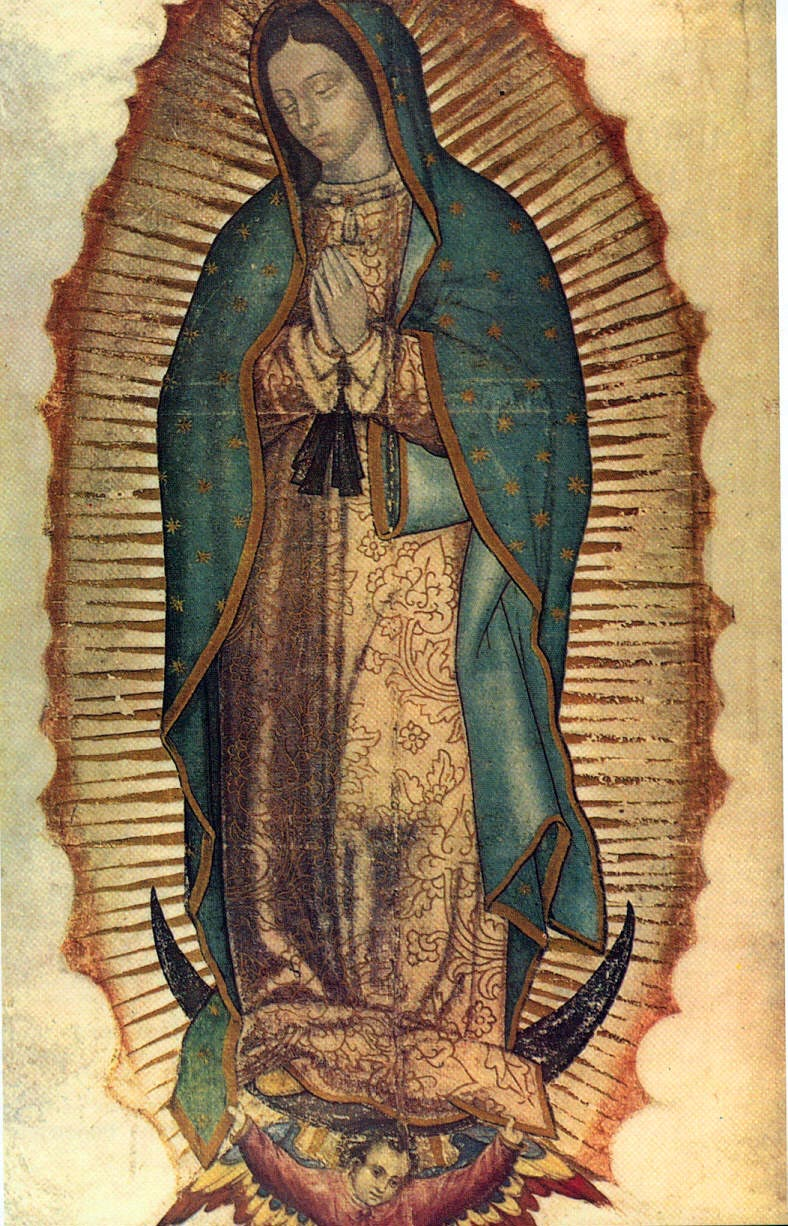
\includegraphics[width=8cm]{virgen.jpg}
\caption{\textit{The sacred image of the Virgin of Guadalupe, from December 1531.  Currently resides in the Shrine of Our Lady of Guadalupe in Mexico City.}  In addition to becoming a religious icon, this symbol has also been a focus of scientific study and a symbol of transition between the past and the modern era in Mexico.}
\end{figure}
\end{document}
